\chapter{Design}

Bei der Entwicklung wurden diverse Design-Entscheidungen gef�llt, welche zum Teil bereits in einem Vorprojekt analysiert wurden. Diese sollen in diesem Kapitel aufgelistet und erl�utert werden. 

\section{System�bersicht}
Um die Applikation zu bedienen, setzt der Anwender die Oculus Rift auf und bewegt sich im von der mitgelieferten Kamera erkennbaren Bereich.

Die Leap Motion wird prinzipiell so verwendet, wie von der Herstellerfirma vorgesehen. Das heisst, diese wird mit dem offiziellen Aufsatz \cite{leap} an der Oculus Rift befestigt, und deckt so den frontalen Sichtbereich des Anwenders ab. Dies l�sst sich gut auf Abbildung \ref{fig:systemuebersicht} erkennen.

Ebenfalls erkennbar ist, dass beide Ger�te per USB mit dem Host-Computer verbunden sind und Daten an die jeweiligen Services schicken. Diese Services werden durch die in Unity verwendeten Plugins angesteuert, und die ausgewerteten Daten in IMVR verwendet.

\afterpage {
	\begin{figure}[t!]
		\centering
		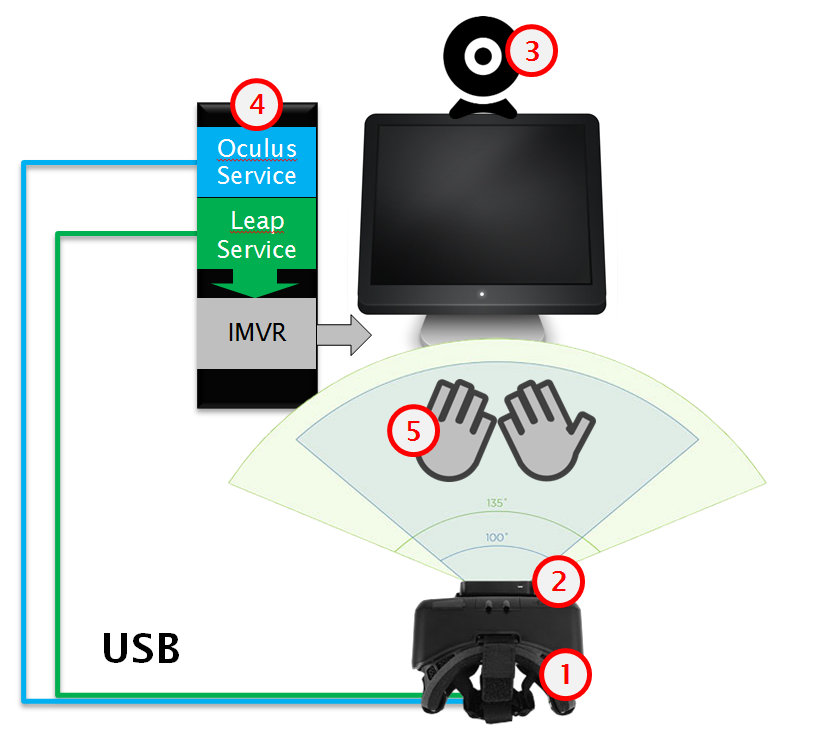
\includegraphics[width=0.8\linewidth]{bilder/systemuebersicht}
		\caption{Eine �bersicht der Technologien und wie sie verbunden sind.}
		\label{fig:systemuebersicht}
	\end{figure}
	
	\begin{table}[H]
		\centering
		\begin{tabular}{p{0.1\linewidth} p{0.3\linewidth} p{0.5\linewidth}}
			\textbf{Nr.} & \textbf{Komponente} & \textbf{Beschreibung} \\ \midrule
			1. & Oculus Rift DK2 & \gls{hmd} f�r den grafischen Output. \\
			2. & Leap Motion & Ger�t, welches H�nde erkennt und ihre Koordinaten an den Computer sendet. \\
			3. & Oculus Rift Kamera & Kamera, welche seit dem DK2 f�r das �rtliche Tracking zust�ndig ist. \\
			4. & Computer & Host-System f�r IMVR. \\
			5. & Benutzer & Benutzer, der die Oculus Rift tr�gt und mit seinen H�nden das Programm steuert. \\
		\end{tabular}
	\end{table}
}

\clearpage

\section{Systemarchitektur}

Zuerst ist es wichtig, zu verstehen, wie die Applikation grob aufgebaut ist. In Abbildung \ref{fig:flow} wird dies in zwei Schritten illustriert.

\begin{figure}[h]
\centering
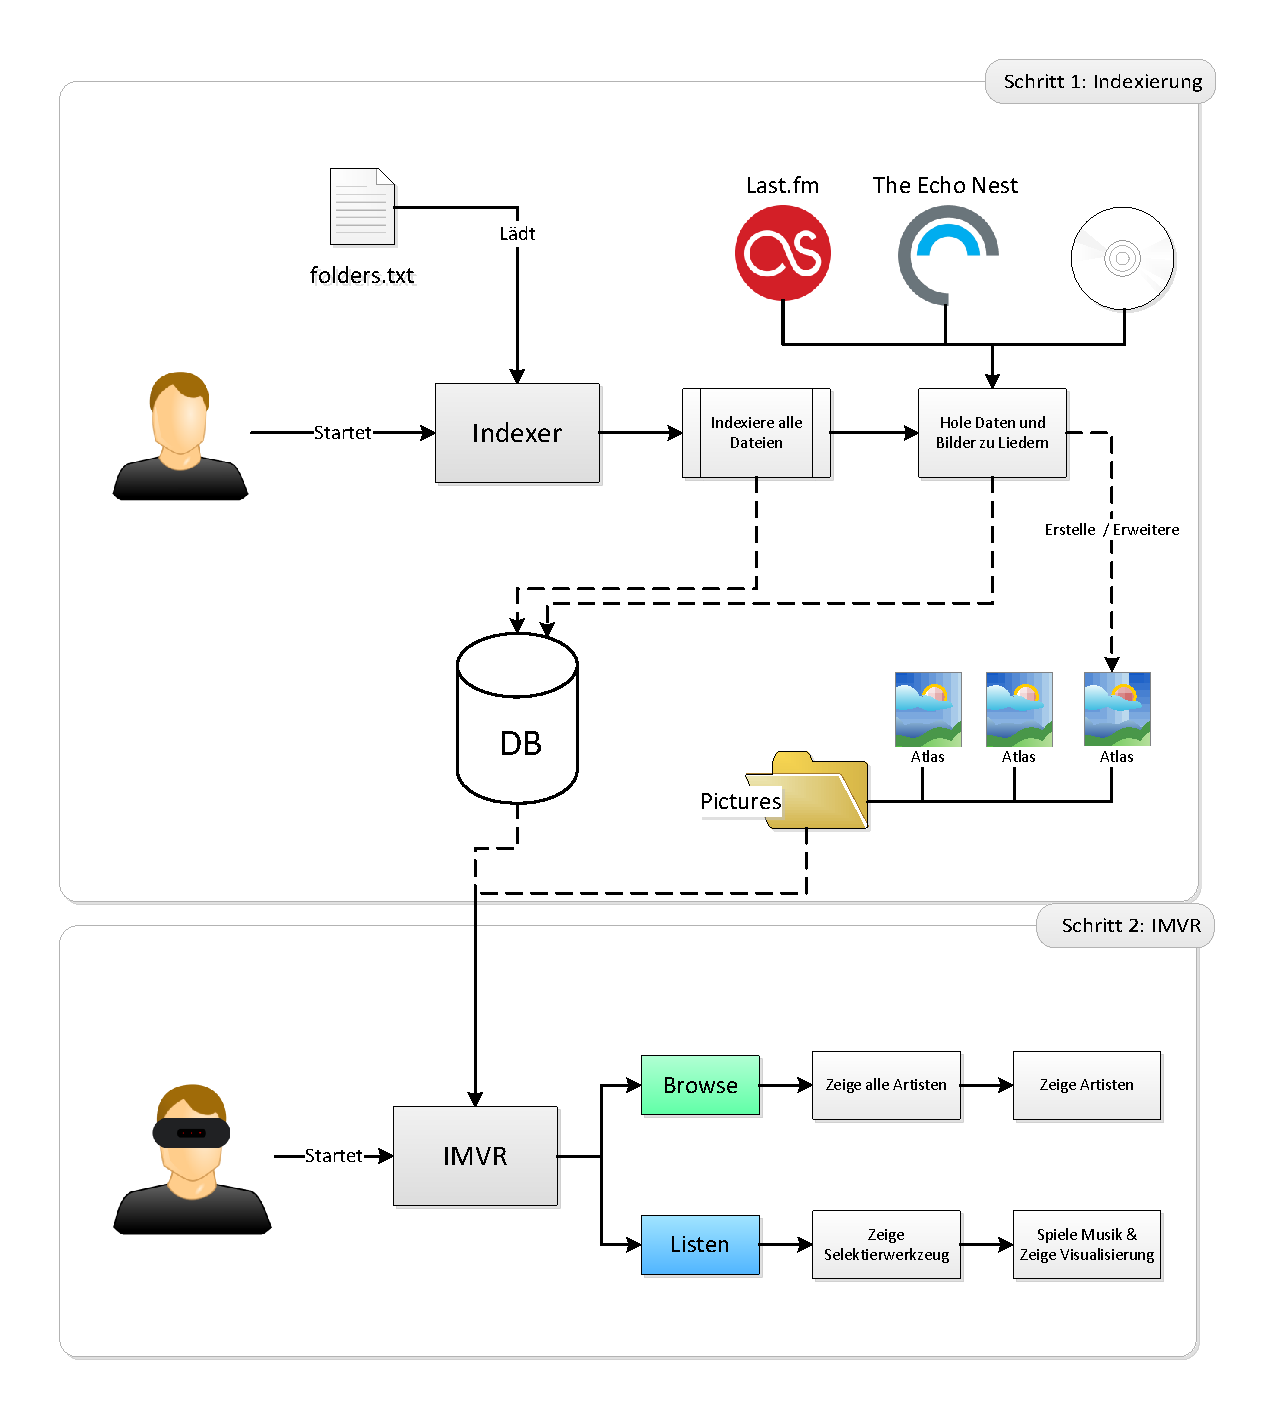
\includegraphics[width=1\linewidth]{diagramme/flow}
\caption{Grober �berblick des Programmablaufs}
\label{fig:flow}
\end{figure}




\section{Systemdesign}

